%%%%%%%%%%%%%%%%%%%%%%%%%%%%%%%%%%%%%%%%%
% Journal Article
% LaTeX Template
% Version 1.4 (15/5/16)
%
% This template has been downloaded from:
% http://www.LaTeXTemplates.com
%
% Original author:
% Frits Wenneker (http://www.howtotex.com) with extensive modifications by
% Vel (vel@LaTeXTemplates.com)
%
% License:
% CC BY-NC-SA 3.0 (http://creativecommons.org/licenses/by-nc-sa/3.0/)
%
%%%%%%%%%%%%%%%%%%%%%%%%%%%%%%%%%%%%%%%%%

%----------------------------------------------------------------------------------------
%	PACKAGES AND OTHER DOCUMENT CONFIGURATIONS
%----------------------------------------------------------------------------------------

\documentclass[twoside,twocolumn]{article}

\usepackage{blindtext} % Package to generate dummy text throughout this template 

\usepackage{graphicx}

\usepackage[sc]{mathpazo} % Use the Palatino font
\usepackage[T1]{fontenc} % Use 8-bit encoding that has 256 glyphs
\linespread{1.05} % Line spacing - Palatino needs more space between lines
\usepackage{microtype} % Slightly tweak font spacing for aesthetics

\usepackage[english]{babel} % Language hyphenation and typographical rules

\usepackage[hmarginratio=1:1,top=32mm,columnsep=20pt]{geometry} % Document margins
\usepackage[hang, small,labelfont=bf,up,textfont=it,up]{caption} % Custom captions under/above floats in tables or figures
\usepackage{booktabs} % Horizontal rules in tables

\usepackage{lettrine} % The lettrine is the first enlarged letter at the beginning of the text

\usepackage{enumitem} % Customized lists
\setlist[itemize]{noitemsep} % Make itemize lists more compact

\usepackage{abstract} % Allows abstract customization
\renewcommand{\abstractnamefont}{\normalfont\bfseries} % Set the "Abstract" text to bold
\renewcommand{\abstracttextfont}{\normalfont\small\itshape} % Set the abstract itself to small italic text

\usepackage{titlesec} % Allows customization of titles
\renewcommand\thesection{\Roman{section}} % Roman numerals for the sections
\renewcommand\thesubsection{\roman{subsection}} % roman numerals for subsections
\titleformat{\section}[block]{\large\scshape\centering}{\thesection.}{1em}{} % Change the look of the section titles
\titleformat{\subsection}[block]{\large}{\thesubsection.}{1em}{} % Change the look of the section titles

\usepackage{fancyhdr} % Headers and footers
\pagestyle{fancy} % All pages have headers and footers
\fancyhead{} % Blank out the default header
\fancyfoot{} % Blank out the default footer
%\fancyhead[C]{Running title $\bullet$ May 2016 $\bullet$ Vol. XXI, No. 1} % Custom header text
\fancyfoot[RO,LE]{\thepage} % Custom footer text

\usepackage{titling} % Customizing the title section

\usepackage{hyperref} % For hyperlinks in the PDF

%----------------------------------------------------------------------------------------
%	TITLE SECTION
%----------------------------------------------------------------------------------------

\setlength{\droptitle}{-4\baselineskip} % Move the title up

\pretitle{\begin{center}\Huge\bfseries} % Article title formatting
\posttitle{\end{center}} % Article title closing formatting
\title{Fast Multiplier Using Booth Encoding} % Article title
\author{%
\textsc{Haocong Wang} \\[1ex] % Your name
%\normalsize University of California \\ % Your institution
\normalsize {mw814@scarletmail.rutgers.edu} % Your email address
%\and % Uncomment if 2 authors are required, duplicate these 4 lines if more
%\textsc{Jane Smith}\thanks{Corresponding author} \\[1ex] % Second author's name
%\normalsize University of Utah \\ % Second author's institution
%\normalsize \href{mailto:jane@smith.com}{jane@smith.com} % Second author's email address
}
\date{\today} % Leave empty to omit a date
\renewcommand{\maketitlehookd}{%
\begin{abstract}
\noindent In this project, we design and implement a 32-bit fast multiplier using booth encoding. We use Verilog to finish the coding of the multiplier. All the codes are finished on EDAplayground. We summary and compare the difference between fast multiplier using booth encoding and other types of multipliers. We test the proposed multiplier with a testbench module. The result shows that our multiplier works fast and well. % Dummy abstract text - replace \blindtext with your abstract text
\end{abstract}
}

%----------------------------------------------------------------------------------------

\begin{document}

% Print the title
\maketitle

%----------------------------------------------------------------------------------------
%	ARTICLE CONTENTS
%----------------------------------------------------------------------------------------

\section{Introduction}

%\lettrine[nindent=0em,lines=3]{B} 
Binary multiplier is one of the basic electronic circuits in digital electronics, such as a computer, to multiply two binary numbers \cite{bi_mul}. As a basic functional unit circuit, multiplier is widely used in various signal processing and conversion circuits. Multiplier can be implemented with a variety of computer arithmetic techniques, which involve computing a set of partial products, and then summing the partial products together.

A binary computer does exactly the same multiplication as decimal numbers do, but with binary numbers. Each long number is multiplied by one digit (either 0 or 1). Therefore, the multiplication of two binary numbers comes down to calculating partial products, shifting them left, and then adding them together.

The method, however, is slow since it involves many intermediate additions, which are time-consuming, so fast multipliers need to developed in order to be adaptive to the increasingly complex computing process. There are various techniques and algorithms to make multipliers faster, such as Wallace tree, BKM algorithm and Kochanski multiplication \cite{bi_mul}. Booth encoding is one of the common methods to calculate multiplication fast and accurately. In this project, we choose booth encoding as our target to design and implement a simple 32-bit fast multiplier using Verilog and EDAplayground as the implementation tools.

%------------------------------------------------

\section{Related Work}~\label{sec:related}

\subsection{Multiplication}

The method for multiplying numbers is based on calculating partial products, shifting them to the left and then adding them together. The most difficult part is to obtain the partial products, as that involves multiplying a long number by one digit. We use binary multiplication as an example to illustrate the process, as shown in figure~\ref{fig:mul}.

\subsection{Booth Encoding}

Booth encoding, or Booth's multiplication algorithm \cite{bo_en}, is a multiplication algorithm that multiplies two signed binary numbers in two's complement notation\footnote{Andrew Donald Booth invented this algorithm in 1950 at Birkbeck College in Bloomsbury, London.}.

Booth's algorithm examines adjacent pairs of bits of the 'N'-bit multiplier Y in signed two's complement representation, including an implicit bit below the least significant bit, $\displaystyle y_{-1} = 0$. For each bit $\displaystyle y_i$, for i running from 0 to N − 1, the bits $\displaystyle y_i$ and $\displaystyle y_{i-1}$ are considered. Where these two bits are equal, the product accumulator P is left unchanged. Where $\displaystyle y_i = 0$ and $\displaystyle y_{i-1} = 1$, the multiplicand times $\displaystyle 2^i$ is added to P; and where $\displaystyle y_i = 1$ and $\displaystyle y_{i-1} = 0$, the multiplicand times $\displaystyle 2^i$ is subtracted from P. The final value of P is the signed product. More details will be given in Section~\ref{sec:des}.

\begin{figure}
	\centering
	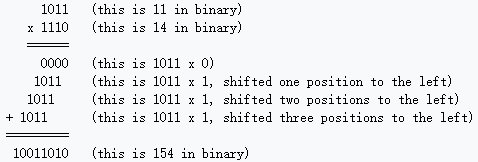
\includegraphics[width=1.0\columnwidth, clip=true]{fig/mul.png}
	\vspace{-4mm}
	\caption{Illustration of the binary multiplication process.}
	\label{fig:mul}
	\vspace{-5mm}
\end{figure}

%------------------------------------------------

\section{Description of Data, Method and Model}~\label{sec:des}

%\begin{itemize}
%\item Donec dolor arcu, rutrum id molestie in, viverra sed diam
%\item Curabitur feugiat
%\item turpis sed auctor facilisis
%\item arcu eros accumsan lorem, at posuere mi diam sit amet tortor
%\item Fusce fermentum, mi sit amet euismod rutrum
%\item sem lorem molestie diam, iaculis aliquet sapien tortor non nisi
%\item Pellentesque bibendum pretium aliquet
%\end{itemize}
%\blindtext % Dummy text

%Text requiring further explanation\footnote{Example footnote}.

In this section, we will discuss the details of the data, method and model used in our project.

\begin{table*}
	\centering
	\begin{tabular}{l|l}
		\toprule
		%\multicolumn{2}{c}{Name} \\
		\cmidrule(r){1-2}
		Multiplicand & Multiplier \\
		\hline
		00000000000000000000000000001111 & 00000000000000000000000000000100 \\
		11111111111111111111111111111111 & 00000000000000000000000000000001 \\
		11111111111111111111111111111111 & 11111111111111111111111111111111 \\
		%John & Doe & $7.5$ \\
		%Richard & Miles & $2$ \\
		\bottomrule
	\end{tabular}
	\caption{Input Data}
    \label{tab:input}
\end{table*}

\subsection{Data}

In our project, we choose 32-bit binary numbers as our input data and therefore, the output will be 64-bit binary numbers. We consider two scenarios, which are unsigned numbers and signed numbers \cite{booth1951signed}. We consider the boundary conditions and choose 3 groups of multiplicands and multipliers, as shown in table~\ref{tab:input}

\subsection{Method}

As mentioned in Section~\ref{sec:related}, we provide detailed introduction for the method used in our project, booth encoding, in this section.

Booth algorithm can be implemented by repeatedly adding one of two predetermined values A and S to a product P, then performing a rightward arithmetic shift on P \cite{chandel2013booth}. Suppose m and r be the multiplicand and multiplier, respectively and x and y represent the number of bits in m and r.

First, we determine the values of A and S, and the initial value of P. For A, we fill the most significant bits with the value of m and the remaining y + 1 bits with zeros. For S, we fill the most significant bits with the value of −m in two's complement notation and the remaining y + 1 bits with zeros. For P, we fill the most significant x bits with zeros and then append the value of r to the right of this. Then we fill the least significant bit with a zero.

Second, we determine the two least significant bits of P. If they are 01, we find the value of P + A. If they are 10, we find the value of P + S. If they are 00, we do nothing and use P directly in the next step. If they are 11, we do nothing and use P directly in the next step.

Third, we arithmetically shift the value obtained in the second step by a single place to the right. Let P now equal this new value. we then repeat steps 2 and 3 until they have been done y times and drop the least significant bit from P, which is now the product of m and r.

\subsection{Model}

Here we provide some introduction to our designed model. First we allow users to input two 32-bit binary numbers, a and b, as the multiplier and multiplicand. We set abs\_a and abs\_b to store the absolute value of a and b, which will be used for signed and unsigned scenarios. Then we write Verilog code to perform booth encoding on these two binary numbers including shifting and adding \cite{deng2015synchronous}. The final results will be shown in EPWave.

%------------------------------------------------

\section{Experimental Procedure and Results}

\begin{figure*}
	\centering
	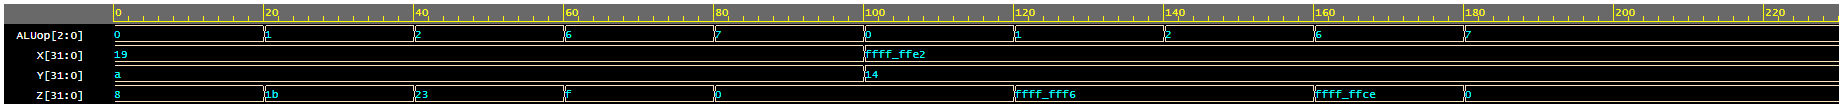
\includegraphics[scale=0.3, clip=true]{../code/EPWave.png}
	\vspace{-2mm}
	\caption{Results of our experiments.}
	\label{fig:ep}
	\vspace{-5mm}
\end{figure*}

\begin{table}
	\centering
	\begin{tabular}{l|l}
		\toprule
		%\multicolumn{2}{c}{Name} \\
		\cmidrule(r){1-2}
		Experiments & Results \\
		\hline
		Exp 1 & 3c \\
		Exp 2 & ffffffff80000001 \\
		Exp 3 & c0000000ffffffff \\
		%John & Doe & $7.5$ \\
		%Richard & Miles & $2$ \\
		\bottomrule
	\end{tabular}
    \caption{Results}
	\label{tab:res}
\end{table}

We use Verilog to write two modules. One is the designation of the multiplier and another one is the test bench. All the codes are finished on EDAplayground. As mentioned in Section~\ref{sec:des}, we use three groups of multiplicands and multipliers to test our designed multiplier, which are shown in table~\ref{tab:input}. We include the EPWave of the test bench in figure~\ref*{fig:ep}. The last line of EPWave shows the result of each group.

In order to make it clear to review, we also add a table to show the results, as shown in table~\ref{tab:res}. We use hexadecimal numbers to represent the products. The result of each multiplication is correct, which means our proposed multiplier is accurate and finish the calculation fast.

%\begin{equation}
%\label{eq:emc}
%e = mc^2
%\end{equation}

%------------------------------------------------

\section{Conclusion}

In this project, we implement a fast multiplier using booth encoding. We finish the designation with Verilog on EDAplayground. The test results show that our product can finish calculation fast and accurately. % Dummy text

%----------------------------------------------------------------------------------------
%	REFERENCE LIST
%----------------------------------------------------------------------------------------

%\begin{thebibliography}{99} % Bibliography - this is intentionally simple in this template

\bibliographystyle{abbrv}
\bibliography{bib}

%\bibitem[Figueredo and Wolf, 2009]{Figueredo:2009dg}
%Figueredo, A.~J. and Wolf, P. S.~A. (2009).
%\newblock Assortative pairing and life history strategy - a cross-cultural
%  study.
%\newblock {\em Human Nature}, 20:317--330.
 
%\end{thebibliography}

%----------------------------------------------------------------------------------------

\end{document}
